\begin{frame}
\frametitle{Introducci\'on}
Se tiene un sistema clasificador con distintos modelos en paralelo que pueden ver features distintas de los datos. Luego se fusionan sus resultados mediante alg\'un m\'etodo, resultando en un \'unico resultado del sistema. Est\'a enfocado particularmente en clasificaci\'on binaria.
\end{frame}



\begin{frame}
\frametitle{Introducci\'on}
\begin{center}
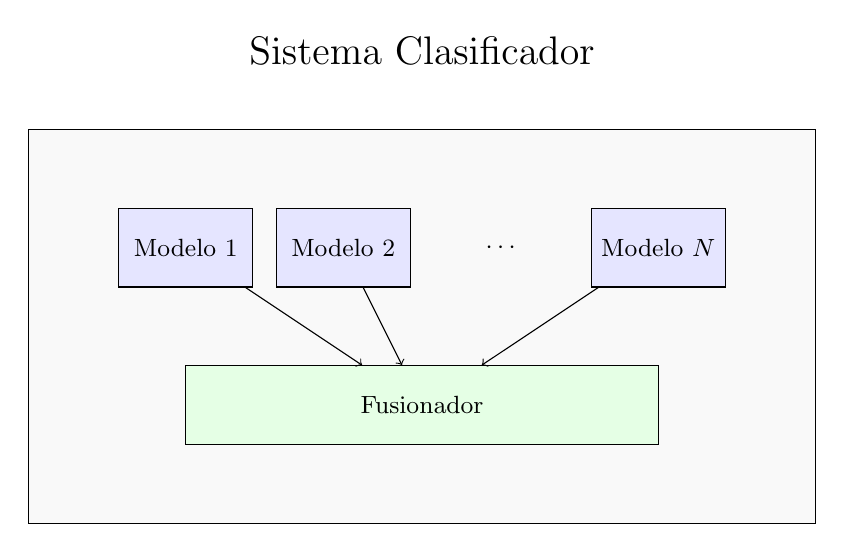
\begin{tikzpicture}[
    every node/.style={font=\small},
    modelo/.style={draw, fill=blue!10, minimum width=1.7cm, minimum height=1cm},
    fusionador/.style={draw, fill=green!10, minimum width=6cm, minimum height=1cm},
    sistema/.style={draw, fill=gray!5}
]
% Sistema
\node[sistema, minimum width=10cm, minimum height=5cm] (sistema) at (0,0) {};
\node[font=\Large] (titulo) at (0,3.5) {Sistema Clasificador};
% Modelos
\node[modelo] (modelo1) at (-3,1) {Modelo 1};
\node[modelo] (modelo2) at (-1,1) {Modelo 2};
\node at (1,1) {$\cdots$};
\node[modelo] (modeloN) at (3,1) {Modelo $N$};
% Fusionador
\node[fusionador] (fusionador) at (0,-1) {Fusionador};
% Aristas
\draw[->] (modelo1) to (fusionador);
\draw[->] (modelo2) to (fusionador);
\draw[->] (modeloN) to (fusionador);
\end{tikzpicture}
\end{center}
\end{frame}



\begin{frame}
\frametitle{Introducci\'on}
Se busca evaluar un modelo para ver como este impacta en el rendimiento del sistema. En otras palabras, se quiere poder evaluar que tan bien se espera que funcione el sistema dado que cierto modelo sea usado.
\end{frame}



\begin{frame}
\frametitle{Introducci\'on}
\begin{center}
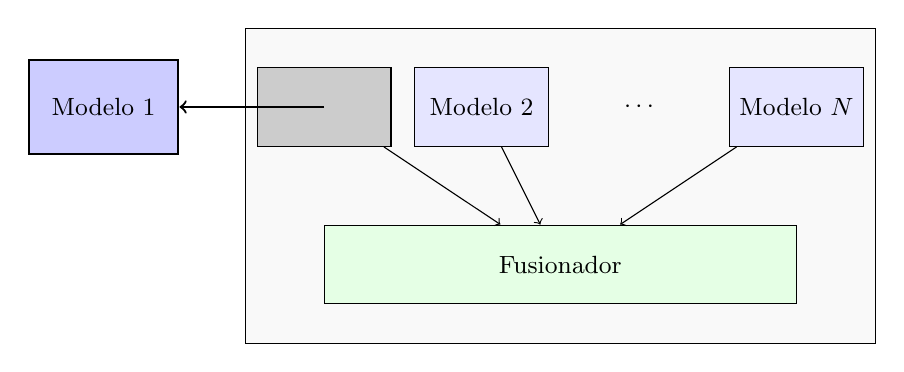
\begin{tikzpicture}[
    every node/.style={font=\small},
    modelo/.style={draw, fill=blue!10, minimum width=1.7cm, minimum height=1cm},
    fusionador/.style={draw, fill=green!10, minimum width=6cm, minimum height=1cm},
    sistema/.style={draw, fill=gray!5}
]
% Modelo externo
\node[modelo, fill=blue!20, thick, minimum width=1.9cm, minimum height=1.2cm] (modeloEvaluar) at (-5.8,1) {Modelo 1};
% Sistema
\node[sistema, minimum width=8cm, minimum height=4cm] (sistema) at (0,0) {};
% Modelos
\node[modelo, fill=gray!40] (modelo1) at (-3,1) {};
\node[modelo] (modelo2) at (-1,1) {Modelo 2};
\node at (1,1) {$\cdots$};
\node[modelo] (modeloN) at (3,1) {Modelo $N$};
% Fusionador
\node[fusionador] (fusionador) at (0,-1) {Fusionador};
% Aristas
\draw[->] (modelo1) to (fusionador);
\draw[->] (modelo2) to (fusionador);
\draw[->] (modeloN) to (fusionador);
\draw[->, thick] (-3,1) to (modeloEvaluar);
\end{tikzpicture}
\end{center}
\end{frame}



\begin{frame}
\frametitle{Informaci\'on disponible}
Datos de los que se dispone para el problema:\\
\vspace{3mm}
\begin{itemize}
\item El sistema incompleto, sin el modelo
\item Datos para la evaluaci\'on del sistema
\item Una funci\'on que asocia las confusiones posibles del sistema a costos
\item El modelo que se pretende evaluar
\item Datos para la evaluaci\'on del modelo
\end{itemize}
\end{frame}



\begin{frame}
\frametitle{Problema}
Para evaluar el modelo, una opci\'on es correr el sistema con el modelo y ver que resultados se obtienen. Para esto es necesario que quien tenga el modelo, tambi\'en tenga acceso al sistema. Incluso aunque eso fuera posible, se podr\'ia querer evitar la ejecuci\'on del sistema completo para cada modelo posible que se busque evaluar. \\El objetivo es proponer un m\'etodo que sea de utilidad para comparar potenciales modelos sin la necesidad de evaluar el sistema nuevamente para cada uno.
\end{frame}



\begin{frame}
\frametitle{Sistema ejemplo}
Se usar\'a como ejemplo el siguiente sistema. Se tienen datos de tipo im\'agenes m\'edicas y hist\'oria cl\'inica. El sistema consiste de dos modelos distintos, cada uno con su veredicto que son luego fusionados con alg\'un m\'etodo. El modelo a evaluar en este ejemplo es el modelo que recibe historias cl\'inicas.
\end{frame}



\begin{frame}
\frametitle{Sistema ejemplo}
\begin{center}
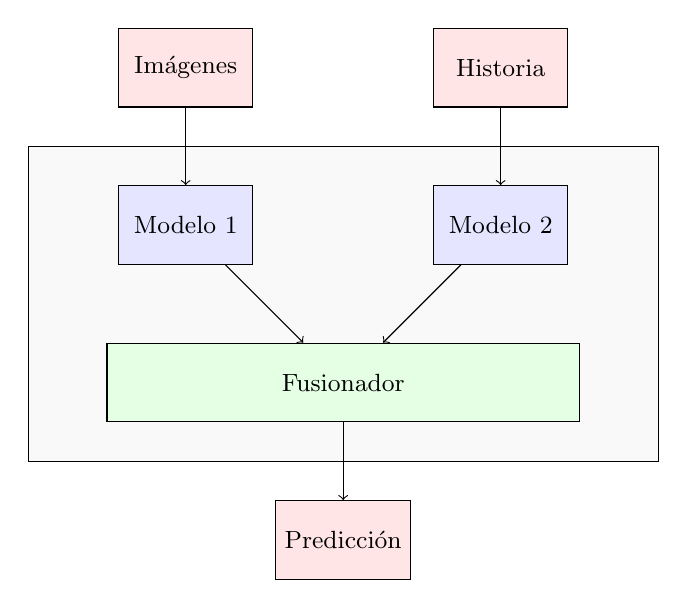
\begin{tikzpicture}[
every node/.style={font=\small},
datos/.style={draw, fill=red!10, minimum width=1.7cm, minimum height=1cm},
modelo/.style={draw, fill=blue!10, minimum width=1.7cm, minimum height=1cm},
fusionador/.style={draw, fill=green!10, minimum width=6cm, minimum height=1cm},
sistema/.style={draw, fill=gray!5}
]
% Datos
\node[datos] (datos1) at (-2,3) {Im\'agenes};
\node[datos] (datos2) at (2,3) {Historia};
% Sistema
\node[sistema, minimum width=8cm, minimum height=4cm] (sistema) at (0,0) {};
% Modelos
\node[modelo] (modelo1) at (-2,1) {Modelo 1};
\node[modelo] (modelo2) at (2,1) {Modelo 2};
% Fusionador
\node[fusionador] (fusionador) at (0,-1) {Fusionador};
% Salida
\node[datos] (resultado) at (0,-3) {Predicci\'on};
% Aristas
\draw[->] (datos1) to (modelo1);
\draw[->] (datos2) to (modelo2);
\draw[->] (modelo1) to (fusionador);
\draw[->] (modelo2) to (fusionador);
\draw[->] (fusionador) to (resultado);
\end{tikzpicture}
\end{center}
\end{frame}



\begin{frame}
\frametitle{Redes Bayesianas}
La forma que se va a utilizar para modelar el problema es mediante una red bayesiana causal. Una red bayesiana causal es un DAG que se usa para representar distribuci\'ones probabilisticas sobre variables no independientes. Se tienen nodos para representar entidades, y aristas que representan causalidad entre esas entidades. Los nodos con doble c\'irculo son determin\'isticos dados los padres.
\end{frame}



\begin{frame}
\frametitle{Redes Bayesianas}
\centering
\begin{tikzpicture}[scale=0.7, every node/.style={font=\tiny}]
% Nodos
\node[draw, fill=blue!30, minimum width=4.2cm, minimum height=3.3cm] at (0,5) (Sistema) {}; 
\node[latent, font=\tiny, fill=green!10] at (0,10) (Persona) {$Persona$};
\node[latent, double, font=\tiny, fill=green!40] at (3.5,8.5) (Clase) {$Clase$};
\node[latent, font=\tiny, fill=green!10] at (-1,8) (Imagen) {$Imagen$};
\node[latent, font=\tiny, fill=green!10] at (1,8) (Historia) {$Historia$};
\node[latent, font=\tiny, fill=blue!20] at (-1,6) (Pred M1) {$Pred^{M1}$};
\node[latent, font=\tiny, fill=blue!20] at (1,6) (Pred M2) {$Pred^{M2}$};
\node[latent, double, font=\tiny, fill=blue!10] at (-2,4) (Conf M1) {$Conf^{M1}$};
\node[latent, double, font=\tiny, fill=blue!10] at (2,4) (Conf M2) {$Conf^{M2}$};
\node[latent, font=\tiny, fill=red!20] at (0,2) (Pred S) {$Pred^S$};
\node[latent, double, font=\tiny, fill=red!10] at (0,0) (Conf S) {$Conf^S$};
\node at (0,3.5) (Fusionador) {\textbf{fusionador}};
\node[font=\large] at (-5.5,5) (Descripcion Sistema) {\color{blue} \underline{Sistema}};
% Aristas
\edge[->] {Persona} {Clase};
\edge[->] {Persona} {Imagen};
\edge[->] {Persona} {Historia};
\draw[->] (Imagen) to node[left] {\textbf{modelo 1}} (Pred M1);
\draw[->] (Historia) to node[right] {\textbf{modelo 2}} (Pred M2);
\edge[->] {Pred M1} {Conf M1};
\edge[->] {Pred M2} {Conf M2};
\edge[->] {Pred M1} {Pred S};
\edge[->] {Pred M2} {Pred S};
\edge[->] {Pred S} {Conf S};
\draw[->] (Clase) to[bend left] (Conf M1.east);
\draw[->] (Clase.280) to[bend left] (Conf M2.north east);
\draw[->] (Clase.south east) to[bend left] (Conf S.east);
\draw[->, very thick, fill=blue, draw=blue] (Descripcion Sistema.east) to (Sistema.west);
\end{tikzpicture}
\end{frame}



\begin{frame}
\frametitle{Intervenci\'on}
En las redes bayesianas existe una operaci\'on interesante llamada intervenci\'on. Esta operaci\'on le asigna a la variable de cierto nodo un valor particular, con probabilidad 1 en todos los casos. Esta operaci\'on se representa en una consulta probabilistica con el operador \textbf{do}. 
\end{frame}



\begin{frame}
\frametitle{Intervenci\'on}
Un ejemplo del operador \textbf{do}:\\
\vspace{3mm}
\begin{minipage}{0.55\textwidth}
\begin{itemize}
\item $P(Y=y | X=x)$
\item $P(Y=y | do(X=x))$
\end{itemize}
\end{minipage}
\begin{minipage}{0.2\textwidth}
\begin{center}
\begin{tikzpicture}
\node[latent] at (0,0.75) (nodeX) {$X$};
\node[latent] at (0,-0.75) (nodeY) {$Y$};
\edge {nodeX} {nodeY};
\end{tikzpicture}
\end{center}
\end{minipage}
\vspace{6mm}\\
La consulta sin \textbf{do} es un condicional normal, donde miramos la probabilidad de $Y=y$ solo para los casos en los que $X=x$.\\
\vspace{1mm}
La consulta con el operador \textbf{do} se realiza sobre toda la distribuci\'on, asumiendo que $X$ vale $x$ siempre. 
\end{frame}



\begin{frame}
\frametitle{Estimaci\'on del costo del sistema}
Para poder comparar entre modelos se separa el proceso en dos partes:\\
\vspace{3mm}
Primero es evaluado el sistema sin el modelo. Se calculan las probabilidades de error y acierto si el modelo hubiera fallado o acertado siempre, usando la operaci\'on de intervenci\'on. \\
\vspace{3mm}
Luego al tener esos valores, se ejecuta un modelo en particular y se intenta estimar alguna m\'etrica del sistema asociada a ese modelo.
\end{frame}



\begin{frame}
\frametitle{Estimaci\'on del costo del sistema}
\begin{itemize}
\item Idealmente, se buscar\'ia estimar el resultado de la evaluaci\'on del sistema si se hubiera corrido con el modelo. Esto no es posible ya que dados distintos modelos con los mismos resultados en su matriz de confusi\'on, es posible que interact\'uen de distintas formas con el sistema y llevar a resultados finales muy distintos.\\
\vspace{3mm}
\item Es por esto que la m\'etrica de inter\'es va a ser que dada la matriz de confusi\'on de un modelo candidato para un conjunto de instancias, estimar el peor resultado posible de la evaluaci\'on del sistema sobre esas instancias. 
\end{itemize}
\end{frame}